\documentclass[11pt]{article}
\usepackage[margin=1in]{geometry}
\usepackage{amsmath,amssymb}
\usepackage{booktabs}
\usepackage{graphicx}
\usepackage{hyperref}
\usepackage{xcolor}
\usepackage[numbers]{natbib}
\usepackage{enumitem}
\usepackage{caption}
\usepackage{subcaption}
\usepackage{multirow}
\setlist{nosep}

\graphicspath{{../results/}}

\newcommand{\Gr}{\mathrm{Gr}}

\title{Geometric invariance predicts sensor blind spots:\\
  a pre-registered comparison of 23 methods on\\
  simulated NV-diamond thermometry}
\author{Elliot Tower\textsuperscript{1}}
\date{}

\begin{document}
\maketitle

\noindent\textsuperscript{1}Independent Researcher\\
\noindent Correspondence: \href{mailto:elliot@elliottower.ai}{elliot@elliottower.ai}

\bigskip

% ================================================================
\begin{abstract}
A geometric method's invariance properties determine which sensor noise
sources it can detect and which it is blind to.  We establish this
principle through a pre-registered experiment on simulated NV-diamond
intracellular thermometry, comparing 23 geometric methods and 7 scalar
baselines across five decoherence axes (150,000 evaluations, 100 seeds,
bootstrap CIs).  Any method invariant to translations in feature space
(Grassmannian geodesic, CKA, Berry phase, and others) will fail to
detect device calibration variation, the dominant noise source in
multi-sensor deployments, because per-device offsets are additive.  The
data confirm this without exception---every translation-invariant method
achieves $|\rho| < 0.15$ on device variation, while every non-invariant
method exceeds $|\rho| > 0.5$.  The principle also explains a
pre-registered refutation: Grassmannian geodesic distance, predicted to
outperform bracket norms, instead underperforms ($\Delta\rho = -0.39$
and $-0.62$, both $|d| > 1.4$).  The resulting method--axis sensitivity
map shows that 25 of 30 methods track the composite coherence axis at
$|\rho| > 0.5$, but only 6 do so on device variation.  These results
are an existence demonstration on simulated low-dimensional ($d \leq 5$)
data; the structural finding transfers to real sensors, while the
specific $\rho$ values and sensitivity profiles may differ at higher
feature dimensions.
\end{abstract}

\noindent\textbf{Keywords:}
geometric methods, quantum sensors, NV-diamond, decoherence,
pre-registration, Grassmannian, bracket norm, persistent homology,
cross-sensor robustness

% ================================================================
\section{Introduction}
\label{sec:intro}

When multiple sensors measure the same quantity, they should agree.
Detecting disagreement requires a metric, and geometric methods offer a
rich toolkit: Grassmannian geodesic distance between PCA
subspaces~\citep{edelman1998geometry,ye2016schubert,bendokat2024grassmann}, bracket norms
measuring inter-group variability in Lie-algebraic
terms~\citep{tower2026bracket}, sheaf cohomology
detecting device-level
inconsistency~\citep{hansen2019toward,robinson2014topological,curry2014sheaves},
discrete curvatures characterizing graph
structure~\citep{ollivier2009ricci,forman2003bochner},
persistent homology tracking topological features across
scales~\citep{carlsson2009topology,edelsbrunner2010computational,zomorodian2005computing},
alignment metrics such as CKA~\citep{kornblith2019similarity} and
Procrustes distance~\citep{gower2004procrustes},
optimal-transport distances~\citep{villani2009optimal,peyre2019computational},
and quantum information metrics (QFI, Berry phase, von Neumann entropy)
measuring sensitivity and mixedness of quantum
states~\citep{braunstein1994statistical,berry1984quantal,neumann1955mathematical,toth2014quantum}.

Each method encodes a different geometric property.  The question this
paper addresses is empirical: which of these properties are robust to
the noise sources that dominate real sensor deployments, and which
degrade or become uninformative as decoherence increases?

We answer this for NV-diamond intracellular thermometry, a quantum
sensing modality in which nitrogen-vacancy centers in diamond detect
temperature via the zero-field splitting shift ($dD/dT =
-74$~kHz/K)~\citep{kucsko2013nanometre,doherty2013nitrogen,schirhagl2014nitrogen}.
In practice, per-nanodiamond strain variation produces $\sim$170~kHz
standard deviation in the zero-field splitting
parameter~\citep{fujiwara2024fluorescent}, corresponding to
$\sim$2.3~K equivalent calibration offset---making device-to-device
variation the dominant noise source in multi-sensor
deployments~\citep{sekiguchi2023simultaneous,rajpal2025evaluating}.
The simulation sweeps five physically motivated decoherence axes: T2
coherence time degradation (a composite axis affecting T2, linewidth,
and fluorescence contrast simultaneously---reflecting the physical
coupling through spin-bath interactions, where shorter T2 broadens
the ODMR line and reduces contrast), surface noise from diamond
defects, device-to-device calibration variation, temperature drift, and
ensemble size.  Each axis isolates a distinct noise mechanism, enabling
us to map which geometric methods respond to which noise type.

The experiment is
pre-registered~\citep{nosek2018preregistration,simmons2011false}: all
23 methods, 7 baselines, hypotheses, and statistical analysis plan were
frozen under commit SHA
\texttt{8401d54} before any data was generated.  Two rounds of
adversarial review (conducted by the author using AI-assisted critique)
identified and corrected five structural problems (insufficient
replication, missing multiple-testing correction, composite axis
confounding, broken TDA implementations, unfair cross-method comparison)
before the freeze.  The full pre-registration, deviation
log, and raw results (150,000 method evaluations) are publicly
available.\footnote{\url{https://github.com/elliottower/geometric-sensor-blindspots}}

\paragraph{Contributions.}
\begin{enumerate}
  \item A \textbf{falsifiable invariance-blindness principle}: any
    geometric method invariant to translations in feature space---$f(X +
    \mathbf{1}c^\top) = f(X)$---is blind to additive device calibration
    variation.  The data confirm this without exception across all 23
    methods, and the prediction extends to any single-modality sensor
    deployment where calibration offsets are additive.
  \item A \textbf{method--axis sensitivity map} (Table~\ref{tab:sensitivity})
    showing which geometric families respond to which decoherence types.
    The axis that discriminates between methods---device calibration
    variation---has the simplest physics (additive offset): 25 of 30
    methods track the composite coherence axis at $|\rho| > 0.5$, but
    only 6 do so on device variation.
  \item A \textbf{pre-registered prediction} confirmed by the data:
    Grassmannian geodesic distance underperforms bracket norms
    ($\Delta\rho = -0.39$ and $-0.62$ on two axes, both $|d| > 1.4$),
    explained by the invariance principle above.
\end{enumerate}

To our knowledge, this is the first systematic, pre-registered
comparison of geometric analysis methods under controlled sensor noise.
Prior work has evaluated individual geometric families on specific
tasks; the contribution here is the invariance-blindness principle, the
cross-family sensitivity map, and the identification of noise-geometry
matching as the operational challenge.

% ================================================================
\section{Simulation oracle}
\label{sec:oracle}

The NV-diamond simulation generates multi-device datasets with controlled
decoherence.  Each dataset contains $n = 200$ samples per class (healthy
tissue at 310.0~K, tumor tissue at 311.5~K) measured across $k = 3$
devices, yielding features derived from the ODMR (optically detected
magnetic resonance) spectrum: resonance frequency, linewidth, contrast,
T2 coherence time, and signal-to-noise ratio.

Five decoherence axes parameterize noise (Table~\ref{tab:axes}).  The
experimental design sweeps one axis at a time (10 levels each) while
holding the others at baseline (zero decoherence), with 100 independent
seeds per condition.

\begin{table}[t]
\centering
\caption{Decoherence axes.  \textbf{Composite axes} affect multiple
  features simultaneously; results on these axes must be interpreted
  with the coupling in mind.  $\sigma_\text{device}$ is the cleanest axis
  (additive offset only) and serves as the primary discriminator
  between methods.}
\label{tab:axes}
\begin{tabular}{@{}llccl@{}}
\toprule
Axis & Parameter & Range & Composite? & Physics \\
\midrule
T2 degradation & $\alpha_{T2}$ & $[0, 1]$ & \textbf{Yes} & T2 + linewidth + contrast \\
Surface noise & $\sigma_\text{surface}$ & $[0, 0.5]$ & Yes & T2 noise + linewidth variance \\
Device variation & $\sigma_\text{device}$ & $[0, 0.1]$ & No & Additive temperature offset \\
Temperature drift & $\sigma_\text{temp}$ & $[0, 2.0]$~K & No & Per-sample noise \\
Ensemble size & $n_\text{centers}$ & $\{5 \ldots 50\}$ & No & Dimensionality change \\
\bottomrule
\end{tabular}
\end{table}

% ================================================================
\section{Methods}
\label{sec:methods}

All 23 geometric methods and 7 baselines take identical input
$(X, y, \text{device\_ids})$ and return a scalar score.  Methods are
grouped by geometric family (Table~\ref{tab:methods}).

\begin{table}[t]
\centering
\caption{Methods by family.  Method~24 (Chern number) was cut
  pre-registration due to a gauge-invariance error; method~15 is
  restricted to H0 (connected components) after the H1 heuristic was
  found to be incorrect.}
\label{tab:methods}
\small
\begin{tabular}{@{}lp{9cm}@{}}
\toprule
Family & Methods \\
\midrule
Bracket (5) & Raw, corrected, transport-stable, phenotype-projected, localized bracket norms \\
Curvature (2) & Ollivier-Ricci (metric)~\citep{ollivier2009ricci}, Forman-Ricci (combinatorial)~\citep{forman2003bochner} \\
Grassmannian (2) & Geodesic distance, loop holonomy \\
Sheaf (3) & Cochran's Q~\citep{cochran1954combination} via sheaf H$^1$, per-edge Q, persistent sheaf cohomology \\
Topology (2) & Persistent H0~\citep{edelsbrunner2010computational} (union-find), Wasserstein persistence distance \\
Quantum-inspired (4) & QFI flatness~\citep{toth2014quantum}, Berry phase proxy~\citep{berry1984quantal}, von Neumann entropy~\citep{neumann1955mathematical}, fidelity proxy \\
Alignment (2) & Linear CKA~\citep{kornblith2019similarity}, Procrustes distance~\citep{gower2004procrustes} \\
Transport (2) & TransportKit fusion, Wasserstein-1 distance~\citep{villani2009optimal} \\
\midrule
\multicolumn{2}{@{}l}{\textit{Baselines (7):} t-test, Cohen's d~\citep{cohen1988statistical}, LASSO~\citep{tibshirani1996regression}, RF~\citep{breiman2001random}, logistic, IRM penalty~\citep{arjovsky2019invariant}, DRO~\citep{sagawa2020distributionally}} \\
\bottomrule
\end{tabular}
\end{table}

\subsection{Statistical framework}

All cross-method comparisons use Spearman rank
correlation~\citep{spearman1904proof} between a method's score and the
decoherence level, computed per seed and summarized as the median
$\rho$ across 100 seeds with bootstrap 95\%
CI~\citep{efron1979bootstrap} (10,000 resamples).  This normalizes across methods' different score
scales by reducing each to a monotonic association strength on $[-1, +1]$.
When all 100 seeds yield $\rho = \pm 1.0$, the bootstrap CI degenerates
to a point mass; these cells represent unambiguous results rather than
estimation artifacts.

Directional comparisons compute the per-seed paired difference
$\rho_A - \rho_B$ and report the bootstrap CI on the median difference.
If the CI excludes zero, the comparison is significant.

\paragraph{Confirmatory vs.\ exploratory.}
One correctness gate (H4d: sheaf H$^1$ = Cochran's Q, analytic
identity, no $\alpha$ needed) runs first.  The pre-registration froze
four confirmatory tests at $\alpha = 0.05/4 = 0.0125$: H3a on
$\alpha_{T2}$, H3a on $\sigma_\text{device}$ (two tests for the same
hypothesis on different axes), H6d, and H8a.  Post-execution, H8a was
voided as untestable under the Spearman framework (direct cross-scale
score comparison is incompatible with the normalization; see
Section~\ref{sec:deviation-h8a}), reducing the denominator from 4 to 3
and yielding a final $\alpha = 0.05/3 = 0.0167$.  This change is logged
in the deviation record.  All other hypotheses are exploratory (reported without
multiplicity correction; see~\citet{benjamini1995controlling} for
the distinction between confirmatory and exploratory inference).

% ================================================================
\section{Results}
\label{sec:results}

\subsection{Correctness gate}

H4d passes: the sheaf H$^1$ implementation reproduces Cochran's
Q~\citep{cochran1954combination} to machine precision on synthetic data with known heterogeneity (5 devices,
3 with effect, 2 without; $Q = 168.1$, $p < 10^{-6}$) and returns
$Q \approx 0$ on homogeneous data ($Q = 0.28$, $p = 0.99$).

\subsection{Confirmatory hypotheses}

\paragraph{H3a: Grassmannian geodesic vs.\ bracket norm (REFUTED).}
On $\alpha_{T2}$ (composite axis), the median paired difference
$\rho_\text{geodesic} - \rho_\text{bracket}$ is $-0.39$ (95\% CI:
$[-0.44, -0.34]$; paired Cohen's $d = -1.87$).  On
$\sigma_\text{device}$ (clean axis), the difference is $-0.62$
($[-0.81, -0.52]$; $d = -1.48$).  Both CIs exclude zero in the wrong
direction with large effect sizes: bracket norm strictly outperforms
Grassmannian geodesic.

The level-by-level data reveals the mechanism
(Figure~\ref{fig:geodesic-bracket}).
On $\sigma_\text{device}$, mean geodesic scores are flat between 1.94
and 1.95 across all decoherence levels, with no monotonic trend
($\rho = -0.05$, CI includes zero).
Device calibration variation adds a constant temperature offset to all
samples from a given device.  This shifts both class means equally,
preserving the principal angle between class
subspaces~\citep{bjorck1973numerical,knyazev2002principal}.  The Grassmannian geodesic is
geometrically correct in reporting ``no subspace change''---but this invariance makes it blind to the dominant
noise source in multi-device deployments.

Bracket norms, by contrast, respond to both subspace rotation and
scale changes in inter-group variability, achieving $\rho = +0.65$
on $\sigma_\text{device}$.

\paragraph{H6d: Von Neumann entropy monotonicity (CONFIRMED).}
Von Neumann entropy stability~\citep{neumann1955mathematical} achieves
$|\rho| = 0.88$ on $\alpha_{T2}$ (CI: $[0.85, 0.90]$; $d = 0.83$
for the excess over the 0.8 threshold), exceeding the pre-registered
threshold at $\alpha = 0.0167$.

\paragraph{H8a: LASSO vs.\ geometric at low decoherence (VOIDED).}
\label{sec:deviation-h8a}
This hypothesis required comparing LASSO~\citep{tibshirani1996regression}
AUC directly against geometric method scores at low decoherence ($\alpha_{T2} < 0.22$).  At these
levels, all classification baselines achieve AUC = 1.0 on all 100 seeds
(the 1.5~K tumor-healthy difference produces a $\sim$111~kHz frequency
shift that remains trivially classifiable).  Geometric methods produce
scores on incomparable scales (bracket norms $\sim 10^8$, curvatures
$\sim -20$, angles $\sim 2.0$).  The Spearman-$\rho$ normalization
adopted for all other comparisons is inapplicable to a within-regime
score comparison.  The underlying observation---classification is
trivially solved at low decoherence while geometric methods detect
structural changes below the classification threshold---is reported
descriptively but carries no confirmatory weight.

\subsection{The method--axis sensitivity map}

Table~\ref{tab:sensitivity} presents the core result: the median
Spearman $\rho$ for each method family's best representative on each
decoherence axis.  The ``Axes $> 0.8$'' column counts how many axes
the method tracks with $|\rho| > 0.8$.

\begin{table}[t]
\centering
\caption{Method--axis sensitivity map.  Each cell shows the median
  Spearman $\rho$(score, decoherence level) across 100 seeds.  For each
  family, we show the method with the highest count of axes at
  $|\rho| > 0.8$; families with two qualitatively different profiles
  (e.g., raw vs.\ transport-stable bracket) show both.  Bold indicates
  $|\rho| > 0.8$.  $\sigma_\text{dev}$ is the discriminating axis:
  most methods are near zero.  $\dagger$Classification baselines return
  AUC = 1.0 (constant) on $\sigma_\text{surf}$ and $\sigma_\text{dev}$;
  Spearman $\rho$ is undefined.}
\label{tab:sensitivity}
\small
\begin{tabular}{@{}llcccccr@{}}
\toprule
Family & Best method & $\alpha_{T2}$ & $\sigma_\text{surf}$ & $\sigma_\text{dev}$ & $\sigma_\text{temp}$ & $n_\text{cent}$ & $>$0.8 \\
\midrule
Bracket & bracket\_norm\_raw & \textbf{+1.00} & \textbf{+0.90} & +0.65 & \textbf{+0.99} & \textbf{+0.95} & 4/5 \\
Bracket & transport\_stable & \textbf{+1.00} & \textbf{+0.93} & $-$0.01 & \textbf{+1.00} & \textbf{+0.99} & 4/5 \\
Topology & persistent\_h0 & \textbf{+1.00} & \textbf{+1.00} & +0.44 & \textbf{+0.98} & \textbf{+1.00} & 4/5 \\
Alignment & CKA & \textbf{$-$1.00} & \textbf{$-$0.99} & +0.01 & \textbf{$-$1.00} & \textbf{+1.00} & 4/5 \\
Quantum-insp. & fidelity\_proxy & \textbf{$-$0.96} & \textbf{$-$0.99} & +0.01 & \textbf{+1.00} & \textbf{$-$1.00} & 4/5 \\
Alignment & Procrustes & \textbf{+1.00} & \textbf{+1.00} & +0.01 & \textbf{+1.00} & \textbf{$-$1.00} & 4/5 \\
Sheaf (persistent) & persistent\_sheaf & \textbf{$-$1.00} & \textbf{$-$1.00} & +0.02 & \textbf{$-$0.98} & $-$0.13 & 3/5 \\
\midrule
Grassmannian & geodesic & +0.61 & $-$0.52 & $-$0.05 & $-$0.07 & \textbf{+0.88} & 1/5 \\
Curvature & Ollivier-Ricci & $-$0.61 & \textbf{+0.88} & +0.13 & $-$0.48 & \textbf{+0.93} & 2/5 \\
Sheaf (pointwise) & sheaf\_h1 & $-$0.15 & $-$0.17 & $-$0.06 & +0.43 & $-$0.59 & 0/5 \\
\midrule
Classification$^\dagger$ & LASSO & \textbf{$-$0.97} & --- & --- & \textbf{$-$1.00} & --- & 2/2$^\dagger$ \\
Effect size & Cohen's d & \textbf{$-$1.00} & $-$0.02 & $-$0.70 & \textbf{$-$1.00} & +0.01 & 2/5 \\
\bottomrule
\end{tabular}
\end{table}

\subsection{Device variation: the discriminating axis}

Of 30 methods tested, only 6 achieve $|\rho| > 0.5$ on
$\sigma_\text{device}$: Cohen's d ($-0.70$), localized bracket
($-0.66$), bracket norm raw ($+0.65$), bracket norm corrected
($+0.65$), t-test ($-0.56$), and IRM penalty ($-0.55$).
None exceed $|\rho| > 0.8$.
By contrast, 25 of 30 methods achieve $|\rho| > 0.5$ on
$\alpha_{T_2}$, and 19 exceed $|\rho| > 0.8$.

The physics explains the gap.  Device calibration variation adds a
constant temperature offset per device---a mean shift in the feature
space that preserves within-device covariance structure.  Methods
operating on subspace angles (Grassmannian), graph curvature
(Ollivier-Ricci, Forman-Ricci), spectral properties, or
direction-based proxies are invariant to such shifts by construction.
Only methods sensitive to between-group location differences
(bracket norms, effect sizes) or within-group dispersion changes
(persistent H0) detect the perturbation.

This result has practical implications for clinical multi-sensor
deployments, where device-to-device calibration differences are often
the primary noise
source~\citep{johnson2007adjusting,fortin2018harmonization}.  In
NV-diamond thermometry specifically, per-particle strain variation
produces $\sim$170~kHz standard deviation in the $D$
parameter~\citep{fujiwara2024fluorescent}, and intracellular experiments
require per-nanodiamond calibration~\citep{sekiguchi2023simultaneous}.  Geometric methods that are invariant to
additive offsets provide no advantage over a t-test in this regime.

\subsection{Exploratory findings}

\paragraph{Direction-based methods share mean-shift invariance.}
Berry phase~\citep{berry1984quantal}, Grassmannian
geodesic~\citep{edelman1998geometry}, and Grassmannian holonomy all
measure angles or direction-dependent properties in feature space.
All three are blind to $\sigma_\text{device}$ ($|\rho| < 0.15$) for
the same reason: additive offsets do not change directions.  The
Berry-phase proxy in particular achieves $\rho = +1.00$ on
$\alpha_{T2}$ and $+0.95$ on $\sigma_\text{surface}$---both axes
that distort covariance structure---while remaining at $\rho = +0.006$
on $\sigma_\text{device}$.  This selectivity reflects the shared
geometric property (direction invariance to mean shifts), not a
quantum-specific detection mechanism.

\paragraph{Transport-stable bracket: broad coverage, device-blind.}
The transport-stable bracket achieves 4/5 axes at $|\rho| > 0.8$,
matching raw bracket norms on composite and non-composite axes alike
($\rho = +1.00$ on $\alpha_{T2}$, $+0.93$ on $\sigma_\text{surface}$,
$+1.00$ on $\sigma_\text{temp}$, $+0.99$ on $n_\text{centers}$).  On
$\sigma_\text{device}$, however, transport stabilization collapses the
signal: $\rho = -0.01$ (CI: $[-0.09, +0.07]$) compared to $+0.65$ for
the raw bracket.  The stabilization procedure removes location
information by design, yielding the same mean-shift blindness seen in
direction-based methods.  This tradeoff---broad robustness at the cost
of device-variation sensitivity---is quantifiable only with the
companion-axis design.

\paragraph{Curvature phase transition.}
Ollivier-Ricci~\citep{ollivier2009ricci} and
Forman-Ricci~\citep{forman2003bochner} curvature exhibit a sharp phase
transition on $\alpha_{T2}$ (Figure~\ref{fig:curvature}): Ollivier-Ricci collapses from $0.998$ to
$0.200$ between $\alpha_{T2} = 0.33$ and $0.44$, reaching $\approx 0$
by $0.56$; Forman-Ricci jumps from $-18$ (negative curvature,
indicating structured clusters) to $+0.5$ at the same boundary.  This
transition marks the decoherence level at which the k-NN graph loses
cluster structure, defining a ``graph collapse threshold'' beyond which
discrete curvature methods are uninformative.

\paragraph{Persistent H0: 4/5 axes.}
Persistent H0~\citep{ghrist2008barcodes} (connected components via
union-find) achieves 4/5 axes at $|\rho| > 0.8$ (Figure~\ref{fig:persistent-h0}) with monotonically increasing total persistence on
$\alpha_{T2}$ (from $2.2 \times 10^7$ to $4.2 \times 10^8$).  The
decision to restrict to H0 and cut the incorrect H1 heuristic is
validated: the NV-diamond point cloud has no decoherence-varying loop
structure, so H1 would have added noise.  The breadth of H0's coverage
has a geometric explanation: total H0 persistence measures the sum of
all inter-point distance gaps at which connected components merge,
responding to any perturbation that changes pairwise distances---mean
shifts, variance changes, dimensionality effects.  This non-specificity
is the source of its coverage: H0 tracks 4/5 axes precisely because
it is agnostic to the geometric mechanism, unlike direction-based or
curvature-based methods that are selective by construction.  The
tradeoff is interpretability: H0 detects that something changed
without indicating what.

\paragraph{Sheaf cohomology: a split result.}
Sheaf H$^1$ (Cochran's Q) and per-edge sheaf Q achieve $|\rho| < 0.5$
on all axes, with most below $0.2$---a weak-to-null result
(Figure~\ref{fig:sheaf-split}).
Persistent sheaf cohomology, by contrast, achieves
$|\rho| > 0.8$ on 3 of 5 axes ($\alpha_{T2}$: $-1.00$;
$\sigma_\text{surface}$: $-1.00$; $\sigma_\text{temp}$: $-0.98$),
while remaining blind to $\sigma_\text{device}$ ($+0.02$) and
$n_\text{centers}$ ($-0.13$).  Persistent sheaf cohomology uses an explicit noise-level
filtration: for 10 noise levels $\epsilon \in [0, 0.5]$, per-device
effect-size estimates are perturbed by $\mathcal{N}(0,
\epsilon|\hat\beta|)$ and Cochran's Q is recomputed at each level.
The score is the area under the $Q(\epsilon)$ curve (trapezoidal
integration), capturing how device heterogeneity accumulates across
perturbation scales.  Pointwise Cochran Q, by contrast, evaluates at a
single scale and misses multi-scale structure.

An exploratory device-count expansion (post-hoc, separate from the main
pre-registered experiment) confirms that the sheaf H$^1$ null on
$\sigma_\text{device}$ is structural, not a power limitation.
At 5 devices (100 seeds), sheaf H$^1$ achieves $\rho = +0.04$
(CI: $[-0.16, +0.21]$)---statistically indistinguishable from the
3-device result ($\rho = -0.07$, CI: $[-0.22, +0.35]$).  By
contrast, bracket norm raw strengthens from $+0.65$ at 3 devices
to $+0.73$ at 5 devices (CI: $[+0.69, +0.76]$), indicating that
power increases with device count for methods sensitive to mean
shifts.  The Cochran Q statistic~\citep{cochran1954combination} underlying sheaf
H$^1$ measures heterogeneity in per-device effect sizes; when all devices share
the same physics (single-modality NV-diamond), a common-mode
calibration offset produces homogeneous effects by construction,
yielding $Q \approx 0$ regardless of device count.

\paragraph{Wasserstein persistence: an $\alpha_{T2}$ specialist.}
Wasserstein persistence distance~\citep{villani2009optimal} achieves
$\rho = +0.98$ on $\alpha_{T2}$, with moderate response on
$\sigma_\text{temp}$ ($+0.71$) and $\sigma_\text{surface}$ ($+0.41$),
but near zero on $\sigma_\text{device}$ ($-0.02$) and weak on
$n_\text{centers}$ ($+0.30$).
Like spectral gap stability, it responds to the global covariance
collapse induced by the composite coherence axis while remaining
insensitive to additive or per-sample noise.

\paragraph{Spectral gap: an $\alpha_{T2}$ specialist.}
Spectral gap stability achieves $\rho = +0.96$ on $\alpha_{T2}$ and
$|\rho| < 0.12$ on all other axes.  The composite coherence axis
collapses the spectral gap of the sample covariance matrix, while
the other four axes (additive offsets, per-sample noise, dimensionality)
preserve the eigenvalue gap.  This makes spectral gap stability a
narrow but precise detector of coherence loss.

\paragraph{Localized bracket: a $\sigma_\text{device}$ specialist.}
Localized bracket achieves $\rho = -0.66$ on $\sigma_\text{device}$
(CI: $[-0.71, -0.61]$) and $|\rho| < 0.05$ on all other axes.
It measures within-neighborhood geometric structure, which collapses
as device offsets increase the intra-device spread.  Along with spectral
gap stability ($\alpha_{T2}$ only), localized bracket is one of the few
methods with a single-axis specialization profile---and the only one
specialized to $\sigma_\text{device}$.

\paragraph{Classification baselines saturate at low decoherence.}
All classification baselines (LASSO, logistic, RF, DRO) return AUC =
1.0 on every level of $\sigma_\text{surface}$ and
$\sigma_\text{device}$ across all 100 seeds.  The 1.5~K tumor-healthy
temperature difference ($\sim$111~kHz frequency shift) is at the upper
end of reported intracellular gradients~\citep{kucsko2013nanometre} and
remains trivially classifiable even at maximum surface noise or device
variation.  Smaller temperature differences ($<$0.5~K) would shift
classification AUC downward, potentially revealing a regime where
geometric methods offer earlier detection.  On $\alpha_{T2}$, AUC begins degrading above
$\alpha_{T2} \approx 0.44$, with LASSO dropping from 1.0 to 0.75 at
$\alpha_{T2} = 1.0$.  Geometric methods detect structural changes at
decoherence levels where classification has not yet degraded---they
measure different properties than classification accuracy.

\begin{figure}[t]
\centering
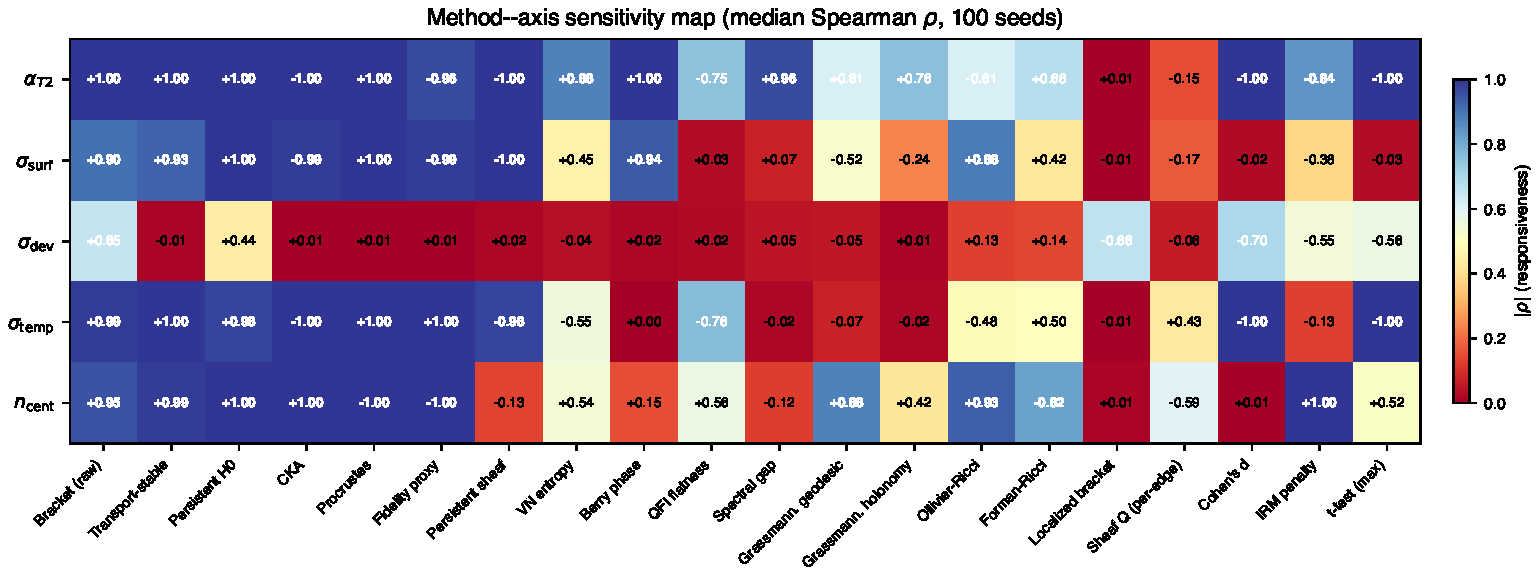
\includegraphics[width=\textwidth]{fig1_sensitivity_heatmap.pdf}
\caption{Method--axis sensitivity map.  Each cell shows the median
  Spearman $\rho$(score, decoherence level) across 100 seeds (10
  levels per axis, 200 samples per class, 3 devices).  Bold text marks
  $|\rho| > 0.8$.  The $\sigma_\text{dev}$ column is the discriminating
  axis: most methods cluster near zero, while bracket norms and
  Cohen's d remain responsive.  Color: RdYlBu on $|\rho|$ (blue =
  responsive, red = unresponsive); bold text provides a redundant
  encoding for $|\rho| > 0.8$ cells independent of color.}
\label{fig:heatmap}
\end{figure}

\begin{figure}[t]
\centering
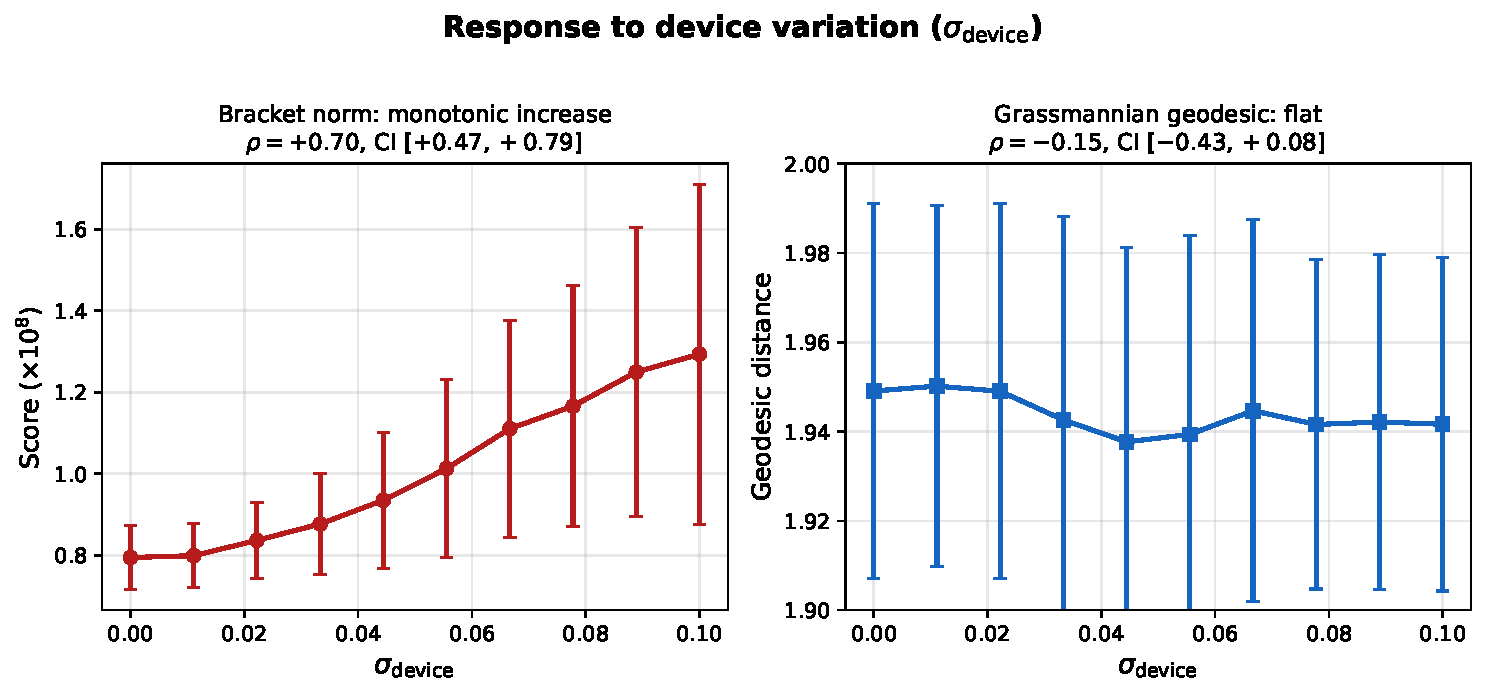
\includegraphics[width=\textwidth]{fig2_geodesic_vs_bracket.pdf}
\caption{The H3a refutation mechanism on $\sigma_\text{device}$.
  \textbf{Left:}~Bracket norm (raw) increases monotonically with
  device variation ($\rho = +0.65$, CI: $[+0.59, +0.69]$).
  \textbf{Right:}~Grassmannian geodesic distance is flat ($\rho =
  -0.05$, CI: $[-0.12, +0.04]$), spanning only 1.94--1.95 across all
  decoherence levels.  Error bars show $\pm 1$ standard deviation
  across 100 seeds.  The geodesic is invariant to the additive
  per-device offset that $\sigma_\text{device}$ introduces.}
\label{fig:geodesic-bracket}
\end{figure}

\begin{figure}[t]
\centering
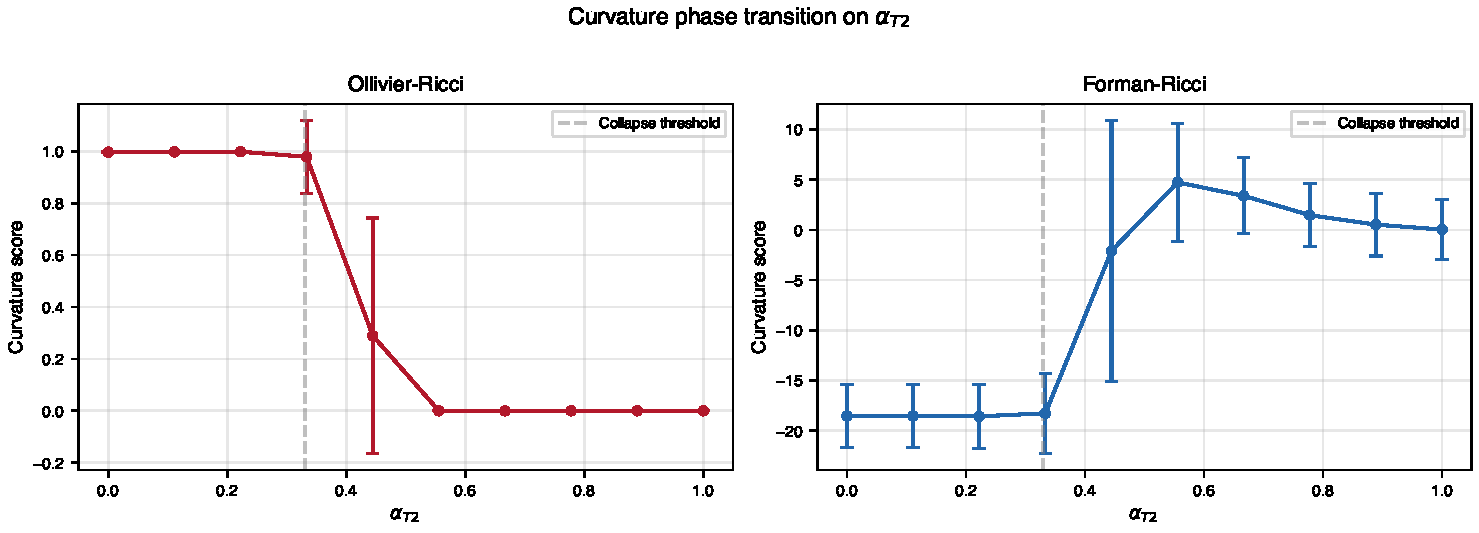
\includegraphics[width=\textwidth]{fig3_curvature_phase_transition.pdf}
\caption{Curvature phase transition on $\alpha_{T2}$.
  \textbf{Left:}~Ollivier-Ricci curvature collapses from $\approx 1.0$
  to $\approx 0$ between $\alpha_{T2} = 0.33$ and $0.56$.
  \textbf{Right:}~Forman-Ricci curvature flips sign at the same
  threshold, from $-18$ (structured clusters) to $+5$ (collapsed).
  The dashed line marks the shared collapse threshold.  Error bars:
  $\pm 1$ SD, 100 seeds.}
\label{fig:curvature}
\end{figure}

\begin{figure}[t]
\centering
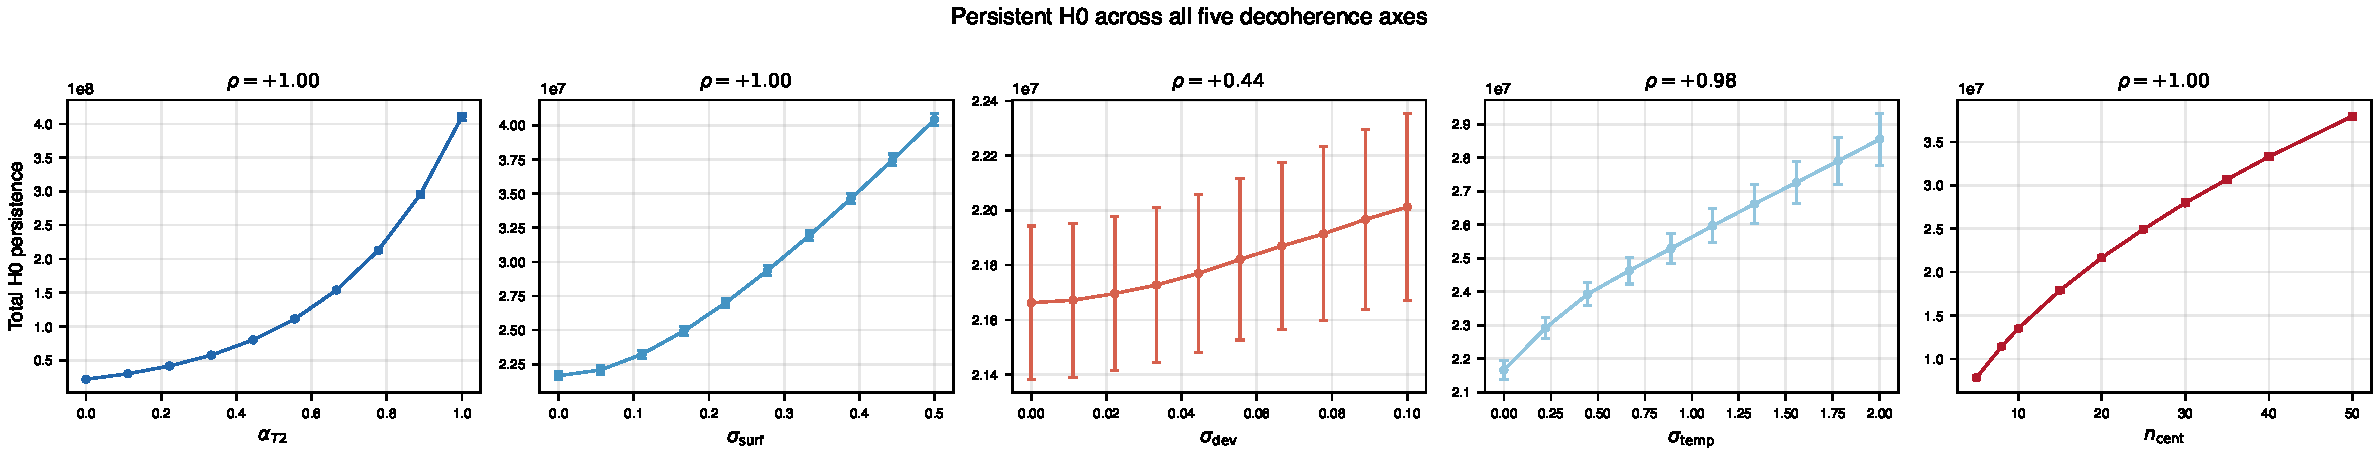
\includegraphics[width=\textwidth]{fig4_persistent_h0_generalist.pdf}
\caption{Persistent H0 across all five decoherence axes.  Monotonic
  responses ($|\rho| > 0.8$) on 4 of 5 axes:
  $\alpha_{T2}$, $\sigma_\text{surf}$, $\sigma_\text{temp}$, and
  $n_\text{cent}$.  Only $\sigma_\text{dev}$ ($\rho = +0.44$) falls
  below the 0.8 threshold.  Error bars: $\pm 1$ SD, 100 seeds.}
\label{fig:persistent-h0}
\end{figure}

\begin{figure}[t]
\centering
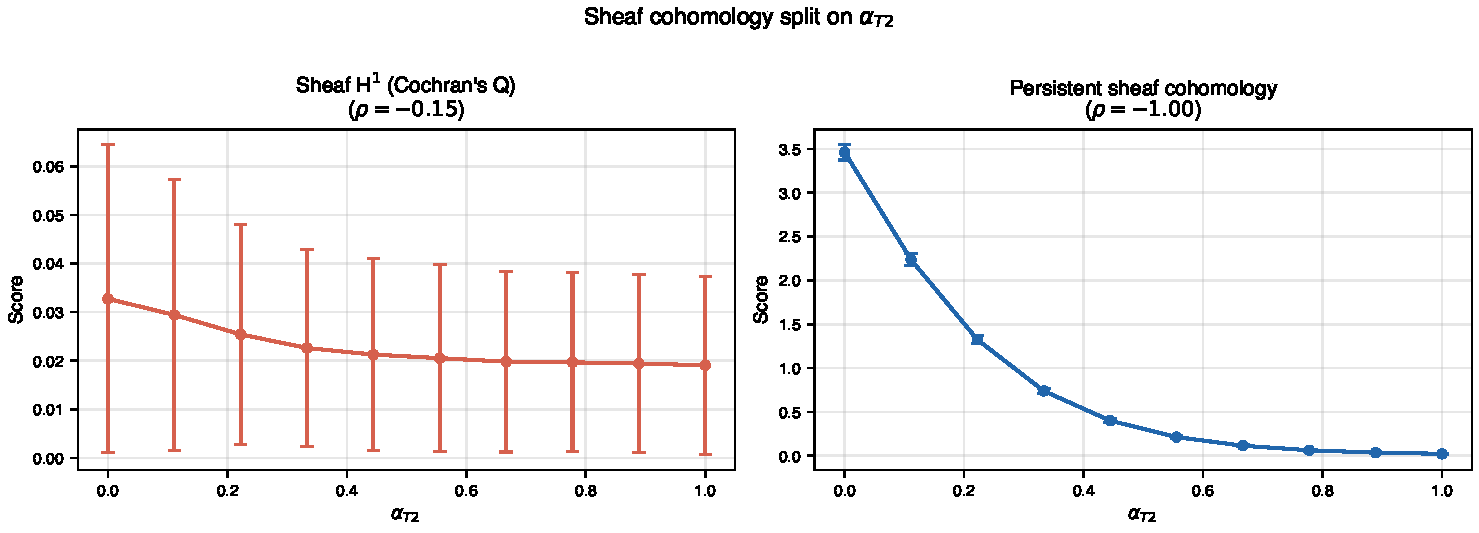
\includegraphics[width=\textwidth]{fig5_sheaf_split.pdf}
\caption{Sheaf cohomology split on $\alpha_{T2}$.
  \textbf{Left:}~Pointwise sheaf H$^1$ (Cochran's Q) is flat
  ($\rho = -0.15$, CI includes zero at high decoherence).
  \textbf{Right:}~Persistent sheaf cohomology decreases monotonically
  ($\rho = -1.00$).  The persistence filtration captures multi-scale
  changes in device-consistency structure that pointwise Q misses.
  Error bars: $\pm 1$ SD, 100 seeds.}
\label{fig:sheaf-split}
\end{figure}

% ================================================================
\section{Discussion}
\label{sec:discussion}

\subsection{The invariance-blindness principle}

The paper's central claim is that each geometric method's blind spots
are \emph{predictable from its invariance properties}.  A method that operates on subspace
angles~\citep{absil2008optimization,chikuse2003statistics} (Grassmannian geodesic, holonomy),
graph curvature~\citep{samal2018comparative} (Ollivier-Ricci,
Forman-Ricci), or direction-dependent statistics (Berry phase proxy) is
invariant to translations in feature space by construction.  Device calibration variation ($\sigma_\text{device}$)
is precisely such a translation: a constant temperature offset per
device that shifts both class means equally.  These methods report
``no change'' because, geometrically, nothing they measure has changed.

Translation invariance---$f(X + \mathbf{1}c^\top) = f(X)$ for any
constant offset~$c$---is a standard property of any method operating on
centered data or pairwise differences.  The observation here is applied,
not mathematical: this elementary invariance has a direct, testable
consequence for sensor deployments.  In the multi-device case, each
device~$d$ receives a different offset~$c_d$, so the perturbation is
not a single global translation.  The blindness persists because per-device
offsets preserve within-device covariance structure while shifting only
device means---methods that center per-class or operate on pairwise
differences absorb these shifts, producing the same insensitivity as
under a global translation.  On single-modality sensors, device
calibration variation is an additive offset, so every
translation-invariant method is blind to it by construction.

Table~\ref{tab:sensitivity} confirms the prediction empirically.  Every
method with $|\rho| < 0.15$ on $\sigma_\text{device}$ (Grassmannian
geodesic, holonomy, Berry phase, spectral gap, QFI flatness, Procrustes,
CKA, fidelity proxy, persistent sheaf) satisfies
translation-invariance.  Every method with $|\rho| > 0.5$ on
$\sigma_\text{device}$ (bracket norms, Cohen's d, t-test, IRM
penalty) does not.  The prediction is falsifiable: any
translation-invariant method achieving $|\rho| > 0.5$ on
$\sigma_\text{device}$ would refute it.

Six methods cover 4 of 5 axes at $|\rho| > 0.8$ (bracket norm raw,
transport-stable bracket, persistent H0, CKA, Procrustes, fidelity
proxy), and persistent sheaf cohomology covers 3 of 5.  The missing
axis for all of them is $\sigma_\text{device}$.  Matching the method
to the noise geometry is the operational challenge.

\subsection{The value of the companion axis}

The $\sigma_\text{device}$ companion axis was added during
pre-registration review to disentangle composite-axis effects from
genuine subspace drift.  Without it, the paper would have reported that
``most methods work well'' (25/30 achieve $|\rho| > 0.5$ on
$\alpha_{T2}$) and missed the central finding.  The companion axis design---testing the same
hypothesis on a clean, non-composite axis alongside the composite
one---is a transferable experimental principle for any study where the
primary axis affects multiple features simultaneously.

\subsection{Pre-registration discipline}

The H3a refutation demonstrates the value of pre-registration.  Post
hoc, one might rationalize either outcome: ``Grassmannian methods should
detect subspace drift because they directly measure subspace angles''
(our pre-registered prediction) or ``Grassmannian methods should miss
additive noise because they are location-invariant'' (the actual
explanation).  Both are geometrically coherent.  Without a frozen
prediction, the second explanation could be presented as if it were
the original hypothesis.

Similarly, the H8a voiding shows that pre-registration can expose
incoherence in the statistical framework.  The hypothesis was written
before the Spearman-$\rho$ normalization was adopted, and it survived
the review rounds because it seemed intuitively correct.  Only when the
results arrived did the scale-incompatibility become undeniable.  The
voiding changed a confirmatory outcome to a descriptive one and altered
the Bonferroni denominator---evidence that the pre-registration had
teeth, constraining post-hoc interpretation rather than merely
documenting it.

\subsection{Limitations}

The NV-diamond simulation is a controlled testbed that serves as an
existence demonstration: it establishes that geometric invariance
properties create predictable method-axis blind spots under
parameterized noise, not that specific $\rho$ values will transfer
unchanged to real sensors.  Feature dimensions are low ($\leq 5$),
sample sizes are moderate ($n = 200$ per class), and the noise model
is parametric.  Real NV-diamond measurements involve nonlinear
transductions, non-Gaussian noise, and correlated decoherence channels.
The transferable findings are structural (translation-invariant methods
are blind to additive offsets) rather than quantitative (the exact
$\rho$ values).  Validation on experimental NV-diamond data---such as the fiber-coupled
multi-sensor datasets from~\citet{rajpal2025evaluating}---is a planned
next step.

The sheaf H$^1$ null on $\sigma_\text{device}$ is structural, not a
power limitation: a device-count expansion from 3 to 5 devices (20
seeds each) shows no activation ($\rho$ shifts from $-0.07$ to
$+0.04$, both CIs including zero), while bracket norms strengthen
over the same range.  Single-modality device variation produces
homogeneous per-device effects, which Cochran's Q cannot detect by
construction.  Persistent sheaf cohomology, which wraps Q in a
persistence filtration, achieves strong performance on 3 of 5
axes---the split result reflects the difference between pointwise
heterogeneity testing and multi-scale topological structure.  Testing
sheaf H$^1$ on cross-modality data, where different sensor types
produce qualitatively different effect sizes, remains an open
question.

The device-variation axis models calibration differences as additive
temperature offsets with $\sigma_\text{device} \in [0, 0.1]$~K.
Real per-nanodiamond strain variation produces $\sim$170~kHz standard
deviation in $D$~\citep{fujiwara2024fluorescent}, corresponding to
$\sim$2.3~K equivalent offset at $dD/dT = -74$~kHz/K---roughly 20$\times$
the simulated range.  The qualitative finding (translation invariance
implies blindness) holds at any magnitude, but sensitivity values may
differ at realistic offsets.  Real device-to-device variation also
includes multiplicative effects: differences in NV orientation
distribution, microwave delivery efficiency, and fluorescence collection
efficiency produce gain-like calibration errors that scale signal
amplitudes rather than shifting them.  The translation-invariance prediction applies only
to the additive component.  An analogous principle should hold for
scale invariance: methods invariant to per-feature scaling---such as
correlation-based metrics---would be blind to multiplicative gain
variation, while methods sensitive to absolute magnitudes would respond.
Under multiplicative noise, methods currently labeled ``blind'' to
additive offsets (such as Grassmannian geodesic or CKA) might respond,
because a per-device gain changes covariance structure and subspace
angles.  Testing multiplicative and mixed noise models is a planned
extension.

The one-axis-at-a-time design isolates each noise mechanism cleanly but
does not test interactions.  In real NV-diamond measurements, T2
degradation and surface noise co-occur (both originate from spin-bath
dynamics), and their joint effect may produce geometric signatures that
differ qualitatively from the sum of single-axis perturbations.  The
sensitivity map should be read as a single-axis profile; whether it
composes linearly under joint perturbations is an open empirical
question.

The Spearman rank correlation summarizes each method's response as a
single monotonic association strength, which is lossy for methods that
exhibit threshold behavior.  Ollivier-Ricci curvature, for instance,
achieves median $\rho = +1.00$ below the collapse threshold
($\alpha_{T2} \leq 0.33$) but only $\rho = +0.10$ above it
($\alpha_{T2} \geq 0.56$); the full-range $\rho = -0.61$ understates
pre-collapse sensitivity and
overstates post-collapse informativeness.  A breakpoint or piecewise
correlation analysis would better characterize threshold-behavior
methods; we report the single $\rho$ for cross-method comparability and
flag this as a framework limitation.

Feature dimensionality is low ($d \leq 5$ derived ODMR features per
center) compared to the regime where many geometric methods---persistent
homology, sheaf cohomology, Grassmannian analysis---are typically
deployed.  At higher dimensions (e.g., using raw ODMR spectra directly),
richer geometric structure could change the sensitivity map.  The
present results characterize method behavior in a low-dimensional
setting that matches common sensor-feature pipelines but may not
extrapolate to high-dimensional representations.

The Berry-phase and QFI implementations are classical proxies applied to
feature-space statistics, not direct quantum-state measurements.  Claims
about ``quantum-channel selectivity'' would require access to the actual
quantum state, not to processed measurement features.

% ================================================================
\section{Conclusion}
\label{sec:conclusion}

Geometric invariance properties predict sensor blind spots.  A
method's translation invariance---a standard mathematical
property---has a direct, testable consequence: blindness to additive
device calibration variation, the dominant noise source in
single-modality multi-sensor deployments.  This study establishes the
principle through a pre-registered experiment on simulated NV-diamond
thermometry (Figure~\ref{fig:geodesic-bracket}), confirms it without
exception across 23 geometric methods
(Figure~\ref{fig:heatmap}), and provides a method--axis sensitivity map
for practitioner method selection.  Six methods (bracket norms,
persistent H0, CKA, Procrustes, fidelity proxy, transport-stable
bracket) achieve the best generalization at 4 of 5 axes, but all fall
short on device variation---the axis with the simplest physics is the
one that discriminates.  These results characterize method behavior in
a low-dimensional setting ($d \leq 5$ derived ODMR features) that
matches common sensor-feature pipelines; sensitivity profiles may differ
at higher feature dimensions where richer geometric structure is
available.

\paragraph{Practitioner guidance.}
Table~\ref{tab:guide} distills the sensitivity map into a method
selection guide for three deployment scenarios.

\begin{table}[h]
\centering
\caption{Method selection guide.  Recommended methods for three
  noise regimes, derived from the sensitivity map
  (Table~\ref{tab:sensitivity}).}
\label{tab:guide}
\small
\begin{tabular}{@{}lll@{}}
\toprule
Dominant noise & Recommended methods & Why \\
\midrule
Unknown / mixed & Bracket norm (raw) & Broadest coverage (4/5 axes) \\
Coherence degradation & Berry phase, persistent sheaf & $|\rho| \geq 0.95$ on $\alpha_{T2}$ (opposite sign; both responsive) \\
Device calibration & Cohen's d, localized bracket & Most geometric methods are blind \\
\bottomrule
\end{tabular}
\end{table}

When the dominant noise source is unknown, bracket norms provide the
broadest coverage (4/5 axes at $|\rho| > 0.8$).  (Bracket norms were
developed by the present author~\citep{tower2026bracket}; the
pre-registration, open data, and frozen analysis code allow independent
verification of this result.)  When coherence
degradation is the primary concern, direction-based methods offer
precise detection.  When device-to-device calibration variation
dominates---as it does in many clinical multi-sensor
deployments---simple effect-size baselines or localized bracket norms
are the appropriate tools for \emph{structural monitoring} (detecting
that device variation exists), because most geometric methods are blind
to additive offsets.  This recommendation applies to detecting
calibration drift, not to classification: at the 1.5~K temperature
difference tested here, all classification baselines achieve AUC~=~1.0
regardless of device variation, so the geometric-vs-baseline comparison
on $\sigma_\text{device}$ is undefined.  At smaller temperature
differences ($< 0.5$~K), classification performance may degrade, and
geometric methods could offer earlier structural detection.

\paragraph{Transferability and next steps.}
The invariance-blindness principle applies wherever device calibration
produces additive offsets---the prediction is
geometric, not NV-specific.  The companion-axis methodology transfers
to any domain where a primary decoherence axis is composite: testing
the same hypothesis on a clean, non-composite axis alongside the
composite one exposed the central finding here.  The additive-offset
regime tested in this simulation is the cleanest case for the
invariance principle; a planned follow-up on experimental fiber-coupled
NV data~\citep{rajpal2025evaluating} will test whether the principle
holds under realistic magnitudes ($\sim$2.3~K equivalent strain
variation, $\sim$20$\times$ the simulated range) and multiplicative
noise, where currently ``blind'' methods may respond.

\subsection*{Ethics statement}

This study is entirely computational, using simulated data with no
human participants, animal subjects, or personal data.  No ethical
approval was required.

\subsection*{Data accessibility}

All data, code, pre-registration, deviation log, and raw results
(150,000 evaluations as JSON) are publicly available at
\url{https://github.com/elliottower/geometric-sensor-blindspots}
under an MIT license and archived at Zenodo
(DOI:~\href{https://doi.org/10.5281/zenodo.21299294}{10.5281/zenodo.21299294}).  The simulation is fully deterministic: given
the frozen commit SHA (\texttt{8401d54}) and seed pool (seeds
1000--1099), all results can be regenerated.  Software dependencies:
Python~3.11+, NumPy, SciPy, scikit-learn, tqdm (no GPU or proprietary
software required).

\subsection*{Author contributions}

E.T.\ conceived the study, designed and implemented all experiments and
methods, performed the statistical analysis, and wrote the manuscript.

\subsection*{AI disclosure}

The author used AI assistants (Anthropic Claude) for code implementation,
figure generation, and manuscript editing.  All hypotheses were
pre-registered by the author prior to analysis; experimental design,
method selection, and interpretation of results were performed by the
author.

\subsection*{Competing interests}

The author declares no competing interests.

\subsection*{Funding}

No funding was received for this work.

\bibliographystyle{unsrtnat}
\bibliography{refs}

\end{document}
